\documentclass[10pt]{article}

\usepackage[a4paper,margin=1in]{geometry}
\usepackage{amsmath}
\usepackage{booktabs}
\usepackage{tikz}
\usetikzlibrary{arrows.meta,positioning}

\title{FloodSim Phase 1: A Toy-Grid Rainfall and Surface Routing Simulator}
\author{FloodSim Project}
\date{\today}

\begin{document}

\maketitle

\begin{abstract}
FloodSim Phase 1 is a deliberately simplified raster-grid flood simulator designed to stabilize semantics, tests, and exported outputs before the project expands into real-terrain ingestion and richer urban flood behavior. The model applies spatially uniform rainfall to each cell, computes local water-surface height as terrain elevation plus ponded depth, and routes a bounded fraction of water to lower orthogonal neighbors using a shared-grid snapshot. This paper documents the implemented Phase 1 contract, the rainfall and boundary assumptions, the step algorithm, and the main limitations that separate this prototype from a city-scale operational flood product.
\end{abstract}

\section{Purpose and Scope}

The long-term FloodSim product aims to support urban flood workflows for city planners, infrastructure teams, risk analysts, and insurers. Phase 1 does not attempt to solve that entire problem. Instead, it provides a trustworthy kernel with:

\begin{itemize}
    \item explicit rainfall semantics
    \item explicit boundary semantics
    \item deterministic step behavior
    \item stable exported outputs
    \item lightweight automated tests
\end{itemize}

This phase should be read as a software and modeling contract, not as a validated hydrology or hydraulic model.

\section{Model State Variables}

The Phase 1 simulator operates on a regular raster grid. Each cell stores:

\begin{itemize}
    \item terrain elevation $z_{r,c}$ in meters
    \item ponded water depth $h_{r,c}$ in meters
    \item surface height $s_{r,c} = z_{r,c} + h_{r,c}$
\end{itemize}

The current model uses only the four orthogonal neighbors of each cell. Diagonal flow is excluded in Phase 1.

\section{Rainfall Contract}

Rainfall is represented as a uniform intensity $I$ in meters per hour. For a simulation step duration $\Delta t$ in seconds, the rainfall depth injected into every cell during that step is:

\[
\Delta h_{\text{rain}} = I \cdot \frac{\Delta t}{3600}
\]

This is an intensity contract rather than a per-step depth contract. As a result:

\begin{itemize}
    \item changing $\Delta t$ changes the rainfall depth added in each step
    \item multiple short steps accumulate the same rainfall depth as one long step over the same total simulated duration
    \item rainfall is applied before any flow routing during the step
\end{itemize}

\section{Routing Semantics}

After rainfall is injected, the simulator examines each cell using a shared snapshot of the grid state. For cell $(r,c)$ with water depth $h_{r,c}$, the algorithm:

\begin{enumerate}
    \item computes the local surface height $s_{r,c}$
    \item identifies all orthogonal neighbors with strictly lower surface height
    \item computes a capped outflow:
    \[
    q_{r,c} = h_{r,c} \cdot f_{\max}
    \]
    where $f_{\max}$ is the configured maximum outflow fraction
    \item splits that outflow among lower neighbors in proportion to relative surface drop
    \item applies all accumulated cell updates only after the full grid scan completes
\end{enumerate}

The snapshot rule matters: water received by a cell during one step cannot be relayed again until the next step.

\section{Boundary Contract}

Phase 1 exposes boundary handling explicitly in the simulation configuration, but only one mode is currently supported:

\begin{itemize}
    \item Closed: water can move only to in-domain neighbors and cannot leave the raster across an outer edge
\end{itemize}

This is a deliberate simplification. Open edge outflow and more realistic domain handling are deferred to later phases.

\section{Step Algorithm Pseudocode}

\begin{enumerate}
    \item Add uniform rainfall depth to every cell.
    \item Allocate a zero-initialized delta array for all cells.
    \item Scan the grid cell by cell.
    \item Skip cells whose current water depth is zero.
    \item Compute the source-cell surface height.
    \item Collect orthogonal neighbors whose surface height is strictly lower.
    \item If no lower neighbors exist, continue to the next cell.
    \item Compute capped outflow as water depth multiplied by the maximum outflow fraction.
    \item Subtract that outflow from the source-cell delta.
    \item Split the outflow across lower neighbors in proportion to relative surface drop.
    \item Add each neighbor share to the corresponding neighbor delta.
    \item After the full scan completes, apply the delta array back to the grid.
\end{enumerate}

\section{Representative Figures}

\subsection{Orthogonal Routing Schematic}

\begin{figure}[h]
\centering
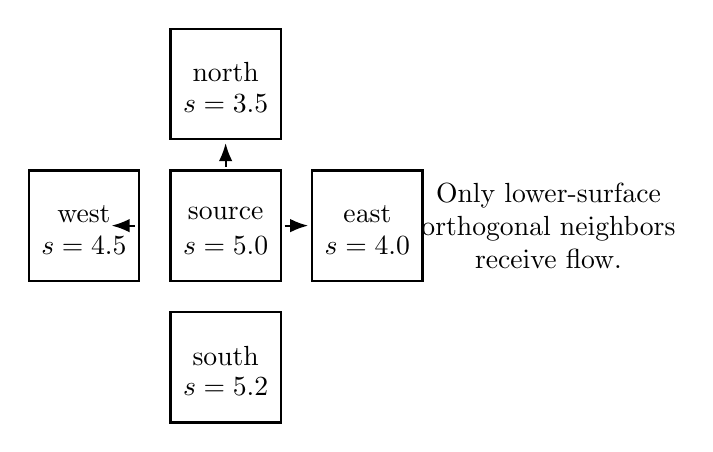
\begin{tikzpicture}[>=Latex,scale=1]
    \draw[thick] (0,0) rectangle (1.4,1.4);
    \draw[thick] (1.8,0) rectangle (3.2,1.4);
    \draw[thick] (-1.8,0) rectangle (-0.4,1.4);
    \draw[thick] (0,1.8) rectangle (1.4,3.2);
    \draw[thick] (0,-1.8) rectangle (1.4,-0.4);

    \node at (0.7,0.85) {source};
    \node at (0.7,0.45) {$s=5.0$};

    \node at (2.5,0.85) {east};
    \node at (2.5,0.45) {$s=4.0$};

    \node at (-1.1,0.85) {west};
    \node at (-1.1,0.45) {$s=4.5$};

    \node at (0.7,2.65) {north};
    \node at (0.7,2.25) {$s=3.5$};

    \node at (0.7,-0.95) {south};
    \node at (0.7,-1.35) {$s=5.2$};

    \draw[->,thick] (1.45,0.7) -- (1.75,0.7);
    \draw[->,thick] (-0.45,0.7) -- (-0.75,0.7);
    \draw[->,thick] (0.7,1.45) -- (0.7,1.75);

    \node[align=center] at (4.8,0.7) {Only lower-surface \\ orthogonal neighbors \\ receive flow.};
\end{tikzpicture}
\caption{Phase 1 routes water only to lower orthogonal neighbors. The south neighbor is excluded because its surface is not lower than the source surface.}
\end{figure}

\subsection{Rainfall Accumulation Graph}

\begin{figure}[h]
\centering
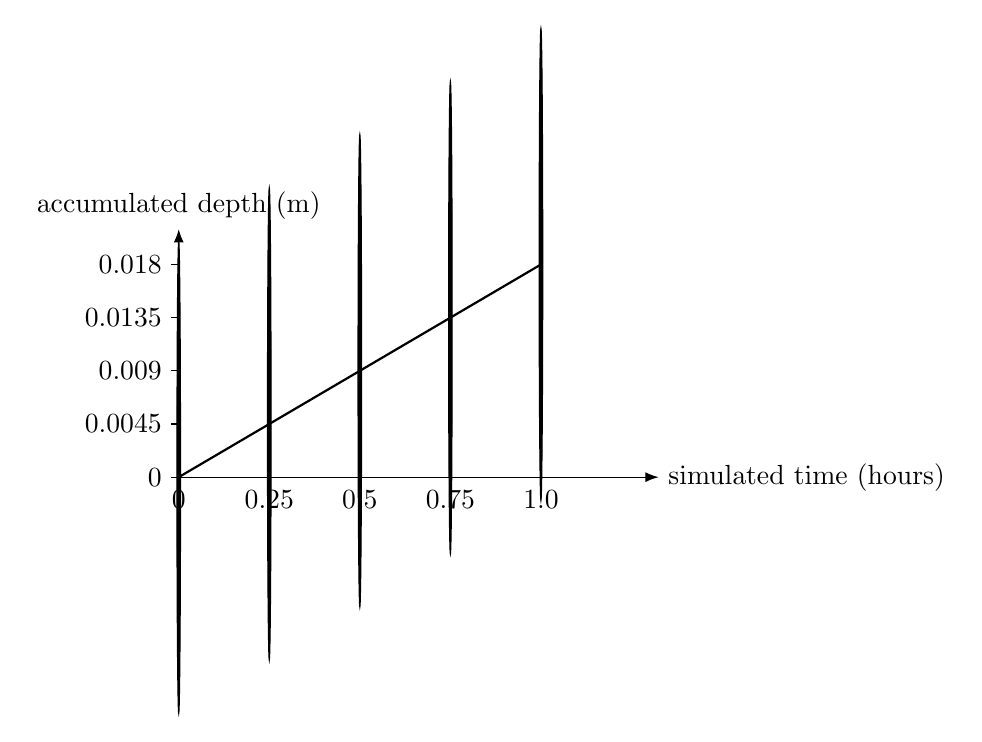
\begin{tikzpicture}[x=1.15cm,y=150cm,>=Latex]
    \draw[->] (0,0) -- (5.3,0) node[right] {simulated time (hours)};
    \draw[->] (0,0) -- (0,0.021) node[above] {accumulated depth (m)};

    \foreach \x/\label in {0/0,1/0.25,2/0.5,3/0.75,4/1.0} {
        \draw (\x,0) -- (\x,-0.00035) node[below] {\label};
    }
    \foreach \y/\label in {0/0,0.0045/0.0045,0.009/0.009,0.0135/0.0135,0.018/0.018} {
        \draw (0,\y) -- (-0.08,\y) node[left] {\label};
    }

    \draw[thick] (0,0) -- (1,0.0045) -- (2,0.009) -- (3,0.0135) -- (4,0.018);
    \filldraw (0,0) circle (0.02);
    \filldraw (1,0.0045) circle (0.02);
    \filldraw (2,0.009) circle (0.02);
    \filldraw (3,0.0135) circle (0.02);
    \filldraw (4,0.018) circle (0.02);
\end{tikzpicture}
\caption{Example accumulation curve for a uniform rainfall intensity of $0.018$~m/h. This is the same contract used by the Phase 1 example run.}
\end{figure}

\section{Exported Outputs}

The Phase 1 export contract is a text CSV with a metadata preamble:

\begin{quote}
\small
{\detokenize{floodsim_csv_version}}, 1 \\
rows, row-count \\
cols, column-count \\
{\detokenize{cell_size_m}}, cell-size-value \\
row, col, {\detokenize{elevation_m}}, {\detokenize{water_depth_m}}, {\detokenize{surface_height_m}}
\end{quote}

This keeps the output self-describing enough for scripts and future viewers while staying lightweight and easy to inspect.

\section{Limitations and Non-Goals}

Phase 1 deliberately does not include:

\begin{itemize}
    \item shallow-water equations or physically rigorous hydrodynamics
    \item infiltration, evaporation, or subsurface processes
    \item storm sewer or drainage network modeling
    \item building blockage or urban roughness treatment
    \item open-boundary or coastal/tidal boundary handling
    \item calibration against observed flood events
\end{itemize}

These omissions are not accidents. They are explicit non-goals of the current phase.

\section{Why Phase 1 Still Matters}

Even with those limitations, this phase is valuable because it locks down:

\begin{itemize}
    \item the meaning of rainfall inputs
    \item the routing contract
    \item the boundary contract
    \item the exported-output contract
    \item a tested baseline for later real-terrain and urban-surface work
\end{itemize}

That makes later phases easier to review and lowers the risk of building DEM import, viewers, and scenario tooling on top of ambiguous behavior.

\section{Conclusion}

FloodSim Phase 1 is best understood as a simulation-core prototype with explicit semantics rather than a finished urban flood product. Its role is to provide a small but stable foundation for subsequent phases: real-terrain ingestion, map-aligned outputs, richer rainfall scenarios, and urban flood behavior that can eventually support practical planning and risk workflows.

\end{document}
